% !TeX program = xelatex
\documentclass[3pt,landscape]{article}
\usepackage{multicol, calc, ifthen, amsmath, amsthm, amsfonts, amssymb, color, graphicx, hyperref, fontspec, xunicode}

\usepackage[landscape]{geometry}

\defaultfontfeatures{Mapping=tex-text,Scale=MatchLowercase}
\ifthenelse{\lengthtest { \paperwidth = 11in}}
    { \geometry{top=.3in,left=.3in,right=.3in,bottom=.3in} }
    {\ifthenelse{ \lengthtest{ \paperwidth = 297mm}}
        {\geometry{top=1cm,left=1cm,right=1cm,bottom=1cm} }
        {\geometry{top=1cm,left=1cm,right=1cm,bottom=1cm} }
    }
\pagestyle{empty}
\makeatletter
\setmainfont{Source Sans Pro}
\setmonofont{Menlo}
\DeclareMathSizes{3}{3}{2}{1}

\renewcommand{\section}{\@startsection{section}{1}{0mm}{-1ex plus -.5ex minus -.2ex}{0.5ex plus .2ex}{\normalfont\large\bfseries}}
\renewcommand{\subsection}{\@startsection{subsection}{2}{0mm}{-1explus -.5ex minus -.2ex}{0.5ex plus .2ex}{\normalfont\normalsize\bfseries}}
\renewcommand{\subsubsection}{\@startsection{subsubsection}{3}{0mm}{-1ex plus -.5ex minus -.2ex}{1ex plus .2ex}{\normalfont\small\bfseries}}
\makeatother
\setcounter{secnumdepth}{0}
\setlength{\parindent}{0pt}
\setlength{\parskip}{0pt plus 0.5ex}
\hypersetup{colorlinks=true, urlcolor=blue}
\def\ci{\perp\!\!\!\perp}

%%%%%%%%%%%%%%%%%%%%%%%%%%%%%%%%%%%%%%%%%%%%%%%%%%

\begin{document}
\raggedright
\footnotesize

\begin{multicols}{3}
\setlength{\premulticols}{1pt}
\setlength{\postmulticols}{1pt}
\setlength{\multicolsep}{1pt}
\setlength{\columnsep}{2pt}

\begin{center}
    \Large{\underline{Algorithms Mini Field Guide}} \\
\end{center}
\begin{center}
    Written by: \href{http://krishna.im}{Krishna Parashar}\\
    Published by: \href{http://www.atrus.co}{Atrus}\\
\end{center}

%%%%%%%%%%%%%%%%%%%%%%%%%

\section*{Basic Properties of Logarithms}
$y = \log _b \left( x \right){\rm{ iff }}x = b^y$\\
$\log _b \left( {xy} \right) = \log _b \left( x \right) + \log _b \left( y \right)$\\
$\log _b \left( x \right) = \log _b \left( c \right)\log _c \left( x \right) = \frac{{\log _c \left( x \right)}}{{\log _c \left( b \right)}}$\\
$\log _b \left( {x^n } \right) = n\log _b \left( x \right)$
$x^a x^b  = x^{\left( {a + b} \right)}$
$\left( {x^a } \right)^b  = x^{\left( {ab} \right)}$
$x^{\left( {\frac{1}{2}} \right)}  = \sqrt x$
$x^{\left( {a - b} \right)}  = \frac{{x^a }}{{x^b }}$

\section*{Basic Series}
Arithmetic Series (Sequential Integers): $\sum\limits_{k = 1}^n {k = \frac{{n\left( {n + 1} \right)}}{2}}$\\
Arithmetic Series (Sequential Odd Ints): $\sum\limits_{k = 1}^n {2k - 1 = n^2 }$\\
Artihmetic Series (Square): $\sum\limits_{k = 1}^n {k^2  = \frac{{n\left( {n + 1} \right)\left( {2n + 1} \right)}}{6}}$
Finite Geometric Series: $\sum\limits_{k = 1}^n {ar^{k - 1}  = \frac{{a\left( {1 - r^n } \right)}}{{1 - r}}}$ \\
Infinite Geometric Series: $\sum\limits_{k = 1}^\infty  {ar^{k - 1}  = \frac{a}{{1 - r}}}$

\section*{Formal Limit Definition of \(O, \Theta, \texttt{and } \Omega\)}
\[\lim_{n \rightarrow \infty}\frac{f(n)}{g(n)}\left\{\begin{array}{lr}
            \geq 0(\infty) & f(n) \in \Omega(g(n))\\
            < \infty(0) & f(n) \in O(g(n))\\
            = c, 0 < c < \infty & f(n) \in \Theta(g(n))
    \end{array}\right.\]

\subsection*{Topological Sort $O(V + E)$}

Constraints: A directed graph G is acyclic if and only if a depth-first search of G yields no back edges. Formally, we say a topological sort of a directed acyclic graph G is an ordering of the vertices of G such that for every edge $(v_i, v_j)$ of G we have $i < j$. If DAG is cyclic then no linear ordering is possible.

\textbf{Topological Sort} returns a list with all nodes pointing left such that basically all parents come before any children (excluding sources).
We order a graph from the \textbf{highest post number} in a decreasing order. \\

Thus we create singly connected component from a DAG with several strongly connected components, each a unique source and unique sink in the DAG. There are multiple topological sorting possible. Used for Runtime Compiling or Scheduling.

\begingroup
    \fontsize{6pt}{6pt}\selectfont
\begin{verbatim}
pre/post 
[u[v v]u] is a Tree/Forward Edge
[v[u u]v] is a Back Edge
[v v][u u] is a Cross Edge
\end{verbatim}
\endgroup

\section*{Master's Theorem}
If
\[T(n)=aT(\lceil n/b \rceil)+O(n^{d}) \texttt{ for } a>0,b>1 \texttt{, and } d\geq 0,\]
then,
\[T(n)=\left\{\begin{array}{lr}
            O(n^{d}) & if d>log_{b}a\\
            O(n^{d}logn) & if d=log_{b}a\\
            O(n^{log_{b}a}) & if d < lob_{b}a\\
        \end{array}
        \right.\]
    Branching Factor: $a$\\
    Depth of Tree = $log_{b}n$\\ 
    Width of Tree: $a^{log_{b}n} = n^{log_{b}a}$

\iffalse
\section*{Volker Strassen}
Divide and conquer matrix multiplication.\\
Matrix multiplication can be broken into subproblems, because it can be performed blockwise. Ex, we can carve X into for \(n/2\) x \(n/2\) blocks
\[X = \begin{bmatrix} A & B \\ C & D \end{bmatrix}, Y = \begin{bmatrix} E & F\\ G & H \end{bmatrix}\]
Then the product can be expressed in terms of those blocks as if the blocks were a single element,
\[XY = \begin{bmatrix} A & B \\ C & D \end{bmatrix} * \begin{bmatrix} E & F\\ G & H \end{bmatrix} = \begin{bmatrix} AE+BG & AF+BH \\ CE+DG & CF+DH \end{bmatrix}\]
The runtime of this recurrence is,
\[T(n)=8T(n/2)+O(n^{2}) \rightarrow O(n^{3})\]
Using clever algebra, this can be improved with integer multiplication, XY can be computed from seven \(n/2\) x \(n/2\) subproblems via decomposition.
\[XY = \begin{bmatrix} P_{5}+P_{4}-P_{2}+P_{6} & P_{1}+P_{2} \\ P_{3}+P_{4} & P_{1}+P_{5}-P_{3}+P_{7} \end{bmatrix}\]
where,
\[\begin{array}{ll}
        P_{1}=A(F-H) & P_{2}=(A+B)H\\
        P_{3}=(C+D)E & P_{4}=D(G-E)\\
        P_{5}=(A+D)(E+H) & P_{6}(B-D)(G+H)\\
        P_{7}=(A-C)(E+F) & \texttt{ }
\end{array}\]
and has a runtime of
\[T(n)=7T(n/2)+O(n^{2}) \rightarrow O(n^{log_{2}7}) \approx O(n^{2})\]
\fi

\section*{Fast Fourier Transform \(O(n\log{n})\)}
The Fast Fourier Transform in the scope of our knowledge thus far is used for Polynomial Multiplication. We want to know the coefficient of $(p \cdot q)(x)$ knowing only the coefficients of $p(x)$ and $q(x)$. The naive way is the one we all use in Algebra which runs in \(O(n^2)\). Here is a faster algorithm:

\begin{enumerate}
  \item Take the coefficients of $p(x)$ and $q(x)$ and plug them into the FFT with the Roots of Unity (We need $2n+1$ points). \(O(n\log{n})\)
  \item From the FFT we get the roots of unity evaluated at $p(x)$ and $q(x)$ and we multiply the respected values from each root together to get $2n+1$ respective pairs of values of $(p \cdot q)(x)$. \(O(n)\)
  \item Finally we interpolate these points using the inverse FFT to get the coefficients of $(p \cdot q)(x)$. \(O(n\log{n})\)
\end{enumerate}
\textbf{Evaluation: }$<values>$ = FFT($<coeff>$, $w$)\\
\textbf{Interpolation: }$<coeff>$ = ($1/n$) FFT($<values>$, $w^{-1}$)\\

\begin{verbatim}
function FFT(A, w)
Input: Coefficient representation of a polynomial A(x)
of degree less than or equal to n−1, 
where n is a power of 2w, an nth root of unity
Output: Value representation A(w_0),...,A(w_n−1)

if w = 1: return A(1)
express A(x) in the form A_e(x^2) + xA_o(x^2)
call FFT(A_e, w^2) to evaluate A_e at even powers of w 
call FFT(A_o, w^2) to evaluate A_o at even powers of w 
for j = 0 to n − 1:
   compute A(w_j) = A_e(w^2j) + w^j A_o(w^2j) 
return A(w_0),...,A(w_n−1)
\end{verbatim}

\iffalse
\textbf{Roots of Unity: }\\
complex \(n^{th}\) roots of unity are given by \(e^{\frac{2 \pi i}{n}}\)
The Vandermonde Matrix,
\[M_{n}(\omega) =
    \begin{bmatrix}
        1 & 1 & 1 & \cdots & 1\\
        1 & \omega & \omega^{2} & \cdots & \omega^{n-1}\\
        1 & \omega^{2} & \omega^{4} & \cdots & \omega^{2(n-1)}\\
        \vdots & \vdots & \vdots & \ddots & \vdots\\
        1 & \omega^{j} & \omega^{2j} & \cdots & \omega^{(n-1)j}\\
        \vdots & \vdots & \vdots & \ddots & \vdots\\
        1 & \omega^{(n-1)} & \omega^{2(n-1)} & \cdots & \omega^{(n-1)(n-1)}
\end{bmatrix}\]
\fi
This process happens recursively. 

\section*{Search Algorithms}

\subsection*{Depth First Search \(O(V + E)\) (Stack)}
Explores all the way down to a tree, then climbs back up and explores alt paths. Use for Topological Sort and Finding Connected Components.
$(pre(u) < pre(v) < post(v) < post(u))$\\

\begin{verbatim}
def explore(G,v): #Where G = (V,E) of a Graph
Input: G = (V,E) is a graph; v ∈ V
Output: visited(u) is set to true for all nodes u 
reachable from v
    visited(v) = true
    previsit(v)
    for each edge(v,u) in E:
        if not visited(u):
            explore(u)
    postvisit(v)

def dfs(G):
    for all v in V:
        if not visited(v):
            explore(v)
\end{verbatim}
\textbf{Previsit} = count till node added to the queue\\
\textbf{Postvisit} = count till you leave the given node\\
A directed Graph has a cycle if and only if it a back edge found during DFS.

\subsection*{Strongly Connected Components $O(n)$}
Us for most edge removal problems, use this to check if still strongly connected.\\
\textbf{Properties: }
\begin{itemize}
\item If the explore subroutine is started at node u, then it will terminate precisely when all nodes reachable from u have been visited.
\item The node that receives the highest post number in a depth-first search must lie in a source strongly connected component.
\item If C and C′ are strongly connected components, and there is an edge from a node in C to a node in C′, then the highest post number in C is bigger than the highest post number in C′.
\end{itemize}
\textbf{Run Time: }$O(n)$\\
\textbf{Big Picture: }Topologically sort the graph; reverse the edges; topologically sort again; ff we reach a new source the resulting traversal is new SCC; continue till end of list. \\

Algorithm:
\begin{itemize}
\item  Run depth-first search on G.\\
\item Run the undirected connected components algorithm (which count uses a counter to count the number of components in G) on G, and during the depth-first search, process the vertices in decreasing order of their post numbers from step 1.
\end{itemize}


\subsection*{Breadth First Search \(O(V + E)\) (Queue)}
\begin{verbatim}
Input: Graph G = (V, E), directed or undirected; vertex s ∈ V 
Output: For all vertices u reachable from s, dist(u) is set
to the distance from s to u.

def bfs(G,s):
    for all u in V:
        dist(u) = infinity
    dist(s) = 0
    Q = [s] (Queue containing just s)
    while Q is not empty:
        u = eject(u)
        for all edges (u,v) in E:
            if dist(v) = infinity:
                inject(Q,v)
                dist(v) = dist(u) + 1
\end{verbatim}


\subsection*{Dijkstra's Algorithm $O(V + E)\log{V}$ (Binary Heap)}
Objective is to find shortest path.
Standard Data Structure is Priority Queue.
\begin{verbatim}
def dijkstra(G,l,s):
    for all u in V:
        dist(u) = infinity
        prev(u) = nil
    dist(s) = 0
    H = makequeue(V) # using dist values as keys
    while H is not empty:
        u = deletemin(H)
        for all edges (u,v) in E:
            if dist(v) > dist(u)+l(u,v)
                dist(v) = dist(u)+l(u,v)
                prev(v) = u
                decreasekey(H,v)
\end{verbatim}

\subsection*{Bellman Ford Algorithm $O(V \cdot E)$}
Objective is to find shortest path allowing for \textbf{negative edges}. 
\begin{verbatim}
procedure shortest-paths(G, l, s)
Input: Directed graph G = (V, E); 
edge lengths {l_e: e in E} with no negative cycles; 
vertex s in V
Output: For all vertices u reachable from s, 
dist(u) is set to the distance from s to u.
for all u in V: 
    dist(u) = infinity 
    prev(u) = nil

dist(s) = 0
repeat |V|-1 times:
    for all e in E: 
        update(e)
\end{verbatim}

\section*{Directed Acyclic Graphs}
\begin{itemize}
    \item Every DAG has a source and sink
    \item A directed graph has a cycle if and only if its depth-first search reveals a back edge.
    \item In a DAG, every edge leads to a vertex with a lower post number.
    \item Every directed graph is a DAG of its strongly connected components.
    \item If the explore subroutine is started at node u, then it will terminate precisely when all nodes reachable from u have been visited
    \item The node that receives the highest post number in a depth-first search must lie in a source strongly connected component
    \item If C and C' are strongly connected components, and there is an edge from a node in C to a node in C', the the highest post number in C is bigger than the highest post number in C'.
    \item In any path of a DAG, the vertices appear in an increasing linearized order allowing you to run Dijkstra's Algorithm in \(O(n)\)
\end{itemize}

\section*{Greedy Algorithms}

\subsection*{Definitions}
A \textbf{Greedy Algorithm} always takes the cheapest least weight edge for its next step, no matter the future consequences.\\
A \textbf{Tree} is an acyclic, undirected, connected graph with $|V| - 1$ edges (or for \textit{MST} exactly $|V| - 1$ edges).\\
A \textbf{Fringe} is all the vertices exactly one hop from you current vertex.\\

\subsection*{Kruskal's MST Algorithm \(O(E\log{E})\)}
\textbf{(If Dense: $|E|$ at most $|V^2|$)}\\
Sort edges using a sorting algorithm then repeatedly add the next lightest edge that doesn't produce a cycle (i.e. only visit new vertices).
\begin{verbatim}
Input: A connected undirected graph G = (V,E) with edge 
        weights w
Output: A minimum spanning tree defined by the edges X

for all u in V:
    makeset(u)
X = {}
Sort the edges E by weight
for all edges {u,v} in E, in increasing order of weight:
    if find(u) != find(v):
        add edge {u,v} to X
        union(u,v)
\end{verbatim}
The above algorithm utilizes disjoint sets to determine whether adding a given edge creates a cycle. Basically by checking whether or not both sets have the same root ancestor.
\begin{center}
    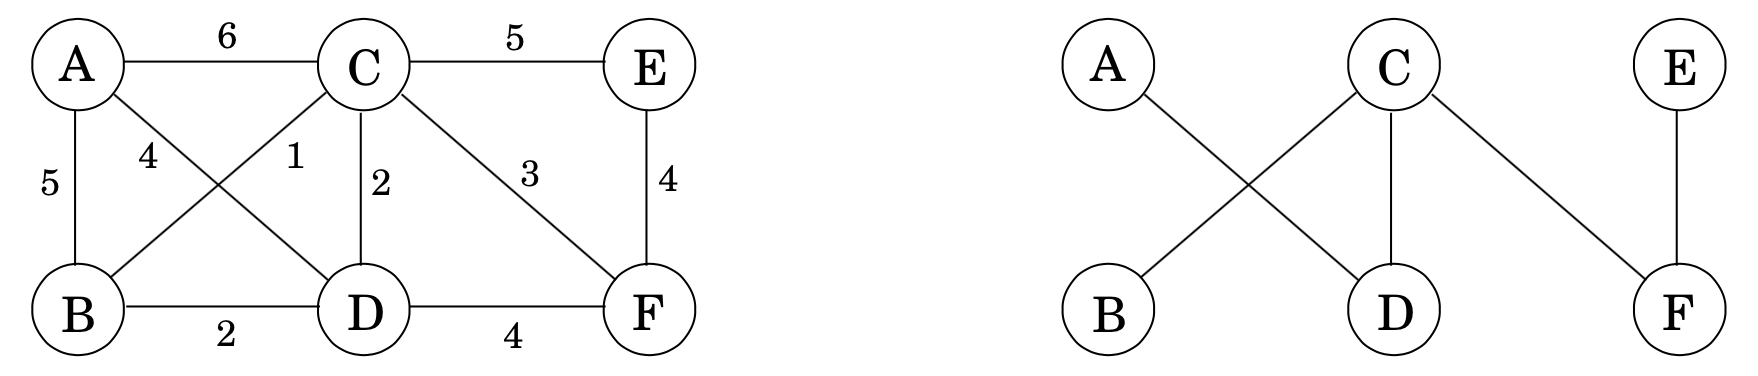
\includegraphics[height=1cm]{images/kruskal-example.png}
\end{center}

\subsection*{Properties of Trees (Undirected Acyclic Graphs)}
\begin{itemize}
    \item A tree with n nodes has n-1 edges
    \item Any connected undirected graph G(V,E), with \(|E|=|V|-1\) is a tree
    \item An undirected graph is a tree if and only if there is a unique path between any pair of nodes.
\end{itemize}

\subsubsection*{Cut Property}
Suppose edges X are part of a minimum spanning tree of \(G=(V,E)\). Pick any subset of nodes S for which X does not cross between S and V-S, and let e be the lightest edge across the partition. Then \(X \cup {e}\) is part of some Minimum Spanning Tree.

\subsection*{Prim's Algorithm \(O(E\log{E})\)}
Objective is to also find the MST.
Alternative to Kruskal's Algorithm; Similar to Dijkstra's)\\
Standard Data Structure is Priority Queue.
\textbf{(If Dense: $|E|$ at most $|V^2|$)}\\
On each iteration, the subtree defined by x grows by one edge, the lightest between a vertex in S and a vertex outside S.

\begin{verbatim}
procedure prim(G, w)
Input: A connected undirected graph G = (V, E) with weights
Output: A minimum spanning tree defined by the array prev
for all u in V : 
    cost(u) = infinity
    prev(u) = nil
Pick any initial node u_0 
cost(u_0) = 0
H = makequeue (V) (priority queue with cost-values as keys) 
while H is not empty:
    v = deletemin(H) 
        for each {v, z} in E:
            if cost(z) > w(v, z): 
                cost(z) = w(v, z) 
                prev(z) = v 
                decreasekey(H, z)
\end{verbatim}
\begin{center}
    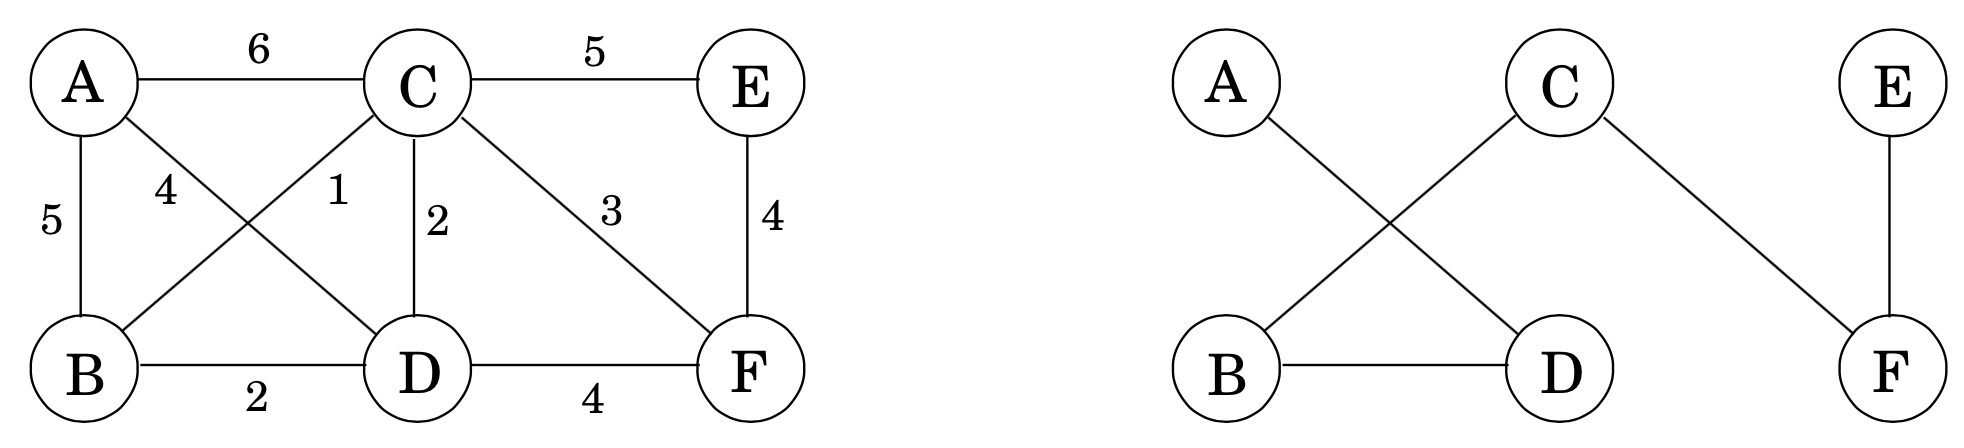
\includegraphics[height=1cm]{images/prims-example.png}
\end{center}


\section*{Set Cover Algorithm (Polynomial Time)}
\begin{verbatim}
Input: A set of elements B; sets S1,...,Sm
Output: A selection of the S_i whose union is B.
Cost: Number of sets picked.

Repeat until all elements of B are covered:
    Pick the set Si with the largest number of
            uncovered elements.
\end{verbatim}

\section*{Disjoint Sets Data Structure}
Contains a function, "find" that returns the root a given set.
$pi$ refers to the parent node.
$rank$ refers to the height subtree hanging form that node (number of levels below it).
\begin{itemize}
\item For any $x, rank(x) < rank(\pi(x))$.
\item Any root node of rank $k$ has at least $2^k$ nodes in its tree.
\item If there are $n$ elements overall, there can be at most $\frac{n}{2^k}$ nodes of rank $k$. The maximum rank is $log n$.
\end{itemize}
\begin{verbatim}
def makeset(x): // O(1)
    pi(x) = x
    rank(x) = 0

def find(x): // O(E log V)
    while x != pi(x):
        x=pi(x)
    return x

def union(x,y): // O(E log V)
    if find(x) == find(y):
        return
    elif rank(find(x)) > rank(find(y)):
        pi(find(y)) = find(x)
    else:
        pi(find(x))=find(y)
        if rank(find(x)) == rank(find(y)):
            rank(find(y)) = rank(find(y)) + 1
\end{verbatim}

\section*{Path Compression}
\begin{verbatim}
function find(x): 
    if x != pi(x): pi(x) = find(pi(x)) 
    return pi(x)
\end{verbatim}
Using path compression allows for an amortized cost of O(1) for out Disjoint Set's $union(x, y)$ and $find(x)$ operations.

\section*{Union Find}
Uses Disjoint Sets Data Structure\\
Runs in per operation $Olog*{n}$ which is the number of times you can take a log of n before it becomes 1 or less. It is very slow and for all practical cases is constant. \\
Basically if find(x) and find(y) return the same value they are in the same graph so do nothing, else add the edge. Then union(x, y).

Union: Worst case is $O(logN)$ Avg for all Ops is $O(nlog*{n})$ where n is number of elements in Data Structure.

%%%%%%%%%%%%%%%%%%%%%%%%%%%%%%%%%%%%%%%%%%%%%%%%%
%%%%%%%%%%%%%%%%%%%%%%%%%%%%%%%%%%%%%%%%%%%%%%%%%
%%%%%%%%%%%%%%%%%%%%%%%%%%%%%%%%%%%%%%%%%%%%%%%%%
%%%%%%%%%%%%%%%%%%%%%%%%%%%%%%%%%%%%%%%%%%%%%%%%%
%%%%%%%%%%%%%%%%%%%%%%%%%%%%%%%%%%%%%%%%%%%%%%%%%

\section*{Huffman Encoding}
A means to encode data using the optimal number of bits for each character given a distribution.
\begin{verbatim}
func huffman(f):
    Input: An array f[1...n] of frequencies
    Output: An encoding tree with n leaves

    let H be a priority queue of integers, ordered by f
    for i=1 to n: insert(H,i)
    for k = n+1 to 2n-1:
        i=deletemin(H), j=deletemin(H)
        create a node numbered k with children i,j
        f[k] = f[i]+f[j]
        insert(H,k)
\end{verbatim}

%%%%%%%%%%%%%%%%%%%%%%%%%

%\section*{Amortized Analysis}

%%%%%%%%%%%%%%%%%%%%%%%%%

\section*{Dynamic Programming}
Fundamentally DP is carefully bruteforcing the solutions to a problem by turning it into smaller and smaller nested subproblems that remember useful information about its bigger or parent subproblem so that it can eventually reconstruct itself to solve the original problem in a reasonable amount of time. This ``remembrance'' is often done using memoization or parent pointers.\\
Dynamic Programming has two approaches, which both have the same asymptotic runtime (differ by a constant):
\begin{enumerate}
\item \textbf{Top Down:}
The top down approach uses the recursive idea of breaking the problem into trivially (but still helpful) smaller subproblems and finding a way (through brute force and memorization) to find the maximum or minimum of every permutation what is be left with ever permutation of the subproblems. This is unlike Divide and Conquer which garners its efficiency from reducing its subproblems to massively smaller problems. 
\item \textbf{Bottom Up:}
The bottom up approach uses the opposite approach of breaking down the problem into its smallest subproblems and iteratively using the smaller problems to solve bigger and bigger problems until it solves the original problem. A table is often used to keep track of these values. BU is more space efficient than TD, unless you use tail recursion for TD.
\end{enumerate} 
You can solve most DP problems by the following steps:
\begin{enumerate}
\item Define the subproblems. Know the \# of subproblems. 
\item Guess a solution for what is not the subproblem (max/min of brute force permutations). Know the \# of guesses.
\item Relate the subproblems to the parent problem. This is the recursive/iterative step. 
\item Do the recursion and memoize or iteratively build a table to keep track of previously used values. These can be used to form a DAG. Ensure the DAG for these are acyclic (i.e. have valid topological order or no dependences on parent problems)
\item Solve the original problem
($\theta(\# subproblems * time/subproblem)$)
\end{enumerate} 
Choosing Subproblems ($i$ is current problem):
\begin{itemize}
\item \textbf{Suffix: } $x[i:] \forall i$ - $O(n)$ (subproblems are broken from i to end)
Topological Order is right to left. 
\item \textbf{Prefix: } $x[:i] \forall i$ - $O(n)$ (subproblems are broken from start to i)
Topological Order is left to right. 
\item \textbf{Substrings: } $x[i:j] \forall i,j$ - $O(n^2)$ (subproblems are fragments of problem, combination of suffix and prefix)
Topological Order is increasing substring size. 
\end{itemize}



\subsection*{Fibonacci \(O(n)\)}
\textbf{Recursive:}
\begin{verbatim}
memo = {}
fib(n):
    if n in memo: return memo[n]
    if n <= 2: f = 2
    else: f = fib(n-1) + fib(n-2)
    memo[n] = f
    return f
\end{verbatim}
\textbf{Iterative:}
\begin{verbatim}
fib = []
fib(n):
    for k in range(1, n):
        if k <= 2: f = 2
        else: f = fib[k-1] + fib[n-2]
        fib[k] = f
    return fib[n]
\end{verbatim}
\subsection*{Shortest Paths $\theta(VE)$}
\textbf{For DAGs:}
For a shortest path (s,v) that uses a limit of, guess take the min of the incoming edge weights into v, say from a node u and then add it to the prefix subproblem of shortest path from (s, u).\\
\textbf{For General: }
$S_k (s, v) = $ weight of shortest path from s to v that uses $\le k$ edges.
$S_k (s, v) = min_{(u, v) in E}(S_{k-1} (s, u) + w(u, v)$\\
This is Bellman-Ford. 

\subsection*{Longest Increasing Subsequence: \(O(n^{2})\)}
Please note that subsequences are any sequences found in another sequences that are not necessarily next to each other (contiguous). Contiguous subsequences are substrings. 
The following algorithm starts at one side of the list and finds the max length of sequences terminating at that given node, recursively following backlinks. Then given all the lengths of paths terminating at that given node choose the max length. Without memoization, this solution would be exponential time.
\begin{verbatim}
L = {}
for j=1,2,...,n:
    L[j] = 1+max{L[i]:(i,j) in E}
    # The (i,j) represents all the edges that go from
    # a node to j.
return max(L)
\end{verbatim}

\subsection*{Edit Distance (Spelling Suggestions)}
This algorithm works by basically choosing the min of the options for every given letter. (The 3 options being adding a gap inbetween letters of one of the strings or matching the two letters and moving on.)\\
ex) Snowy and Sunny have an edit distance of 3 with this configuration
\begin{verbatim}
S _ N O W Y
S U N N _ Y
\end{verbatim}
\begin{verbatim}
for i = 0,1,2,...,m:
    E(i,0) = i
for j = 1,2,...,n:
    E(0,j) = j
for i = 1,2,...,m:
    for j = 1,2,...,n:
        E(i,j) = min{E(i-1,j)+1,E(i,j-1)+1,E(i-1,j-1)
                    +diff(i,j)}
return E(m,n)
\end{verbatim}

\subsection*{Knapsack \(O(nW)\)}
Items have a weight and a value, you want to maximize the value within a given weight. (The amount you can carry in your knapsack)\\
With repetition:
\[K(\omega)=max_{\texttt{items}}\{K(\omega-\omega_{\texttt{item}})+value\}\]
Without repetition:
\[K(\omega,j)=max_{\texttt{available items}}\{K(\omega-\omega_{j},j-1)+V_{j},k(\omega, j-1)\}\]

\subsection*{Parenthesization \(O(n^3)\)}
\[C(i,j)=min\{C(i,k)+c(k+1,j)+m_{i-1}\cdot m_{k} \cdot m_{j}\}\]

\subsection*{Floyd-Warshall \(O(|V|^{3})\)}
Used for finding shortest paths in a weighted graph with positive or negative edge weights (but with no negative cycles/
\begin{verbatim}
for i=1 to n:
    for j=1 to n:
        dist(i,j,0) = infinity
    for all (i,j) in E:
        dist(i,j,0) = l(i,j)
for k = 1 to n:
    for i = 1 to n:
        for j = 1 to n:
            dist(i,j,k) = min{dist(i,k,k-1)+
                              dist(k,j,k-1),
                              dist(i,j,k-1)}
\end{verbatim}

\subsection*{Traveling Salesman Problem (TSP) \(O(n^{2}2^{n})\)}
Shortest path for visiting all nodes. 
\begin{verbatim}
C({1},1)=0
for s = 2 to n:
    for all subsets S in {1,2,...,n} of size s and has l:
        C(S,1) = infinity
        for all j in S,j != 1:
            C(S,j) = min{C(S-{j},i)+dij:i in S,i not in j}
return min over j, C({1,...,n},j)+dj1
\end{verbatim}

%%%%%%%%%%%%%%%%%%%%%%%%%

\section*{Linear Programming}
Feed into a LP solver like Simplex an \textit{Objective Function} which states if you want to maximize or minimize the equation (max$(x+2y)$), \textit{Constraints} which are limitations for the variables of the Objective Function ($x \ge 0, y \le 600$).
\begin{enumerate}
    \item To turn a maximization problem into a minimization (or vice versa) just multiply the coeficients of the objective function by -1.
    \item To turn an inequality constraint like \(\sum_{i=1}^{n}a_i x_i \leq b\) into an equation, introduce a new variable S and use, \(\sum^n_{i=1}a_{i}x_{i}+s = b\), \(s \geq 0\) (S is known as a slack variable)
    \item To change an inequality constraint into inequalities rewrite \(ax=b\),\\
        as \(ax \leq b \texttt{ and } ax \geq b\)
    \item If a linear program has an unbounded value then its dual must be infeasible.
\end{enumerate}

\subsection*{Simplex}
Typically Polynomial time; Worst Case Exponential.
\begin{verbatim}
let v be any vertex of the feasible region
while there is a neighbor v' of v with a better value:
    set v = v'
return v
\end{verbatim}


\subsection*{Max Flow}
Construct graph G that is a simple directed graph with source s and sink t. No negative capacities are possible.\\
Construct a Residual Graph with forward edges for the amount of capacity that is not being used (capacity - current use) and a back edge for what is currently being used. 

\subsubsection*{Ford-Fulkerson}
Start with no flow on your graph. Find a path using DFS. Then create a residual graph. We can now use DFS for finding a path from s to t in the residual graph. If one exists we are not optimally using our flow. We then find the edge with the LEAST capacity edge - this is our bottleneck - and add flow onto all the edges in that path up to the capacity that is not being used by the bottleneck edge, hereby maximizing the flow of the path. Our new flow is guaranteed to be better. Create a new residual graph and repeat until no path in the residual graph can be found from s to t. This will happen when capacity = current use, as we lose our forward edge and only have a back edge.\\
This algorithm will sometimes decrease flow in one area to increase flow in another. Max flow is the total weights of incoming edges to the sink. Runtime would be $O(E * M)$, where $M$ is the number of iterations and $E$ is the time to find a path. This can also be stated as $O($maxflow$*E)$. However this may not terminate. If you use BFS instead of DFS you are using the Edmonds-Karp Algorithm which will terminate and has complexity $O(V*(E)^2)$, which is better for large networks.
\begin{center}
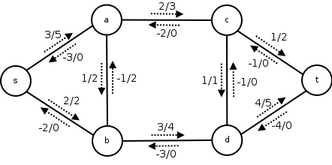
\includegraphics[scale=.25]{images/flow.png}
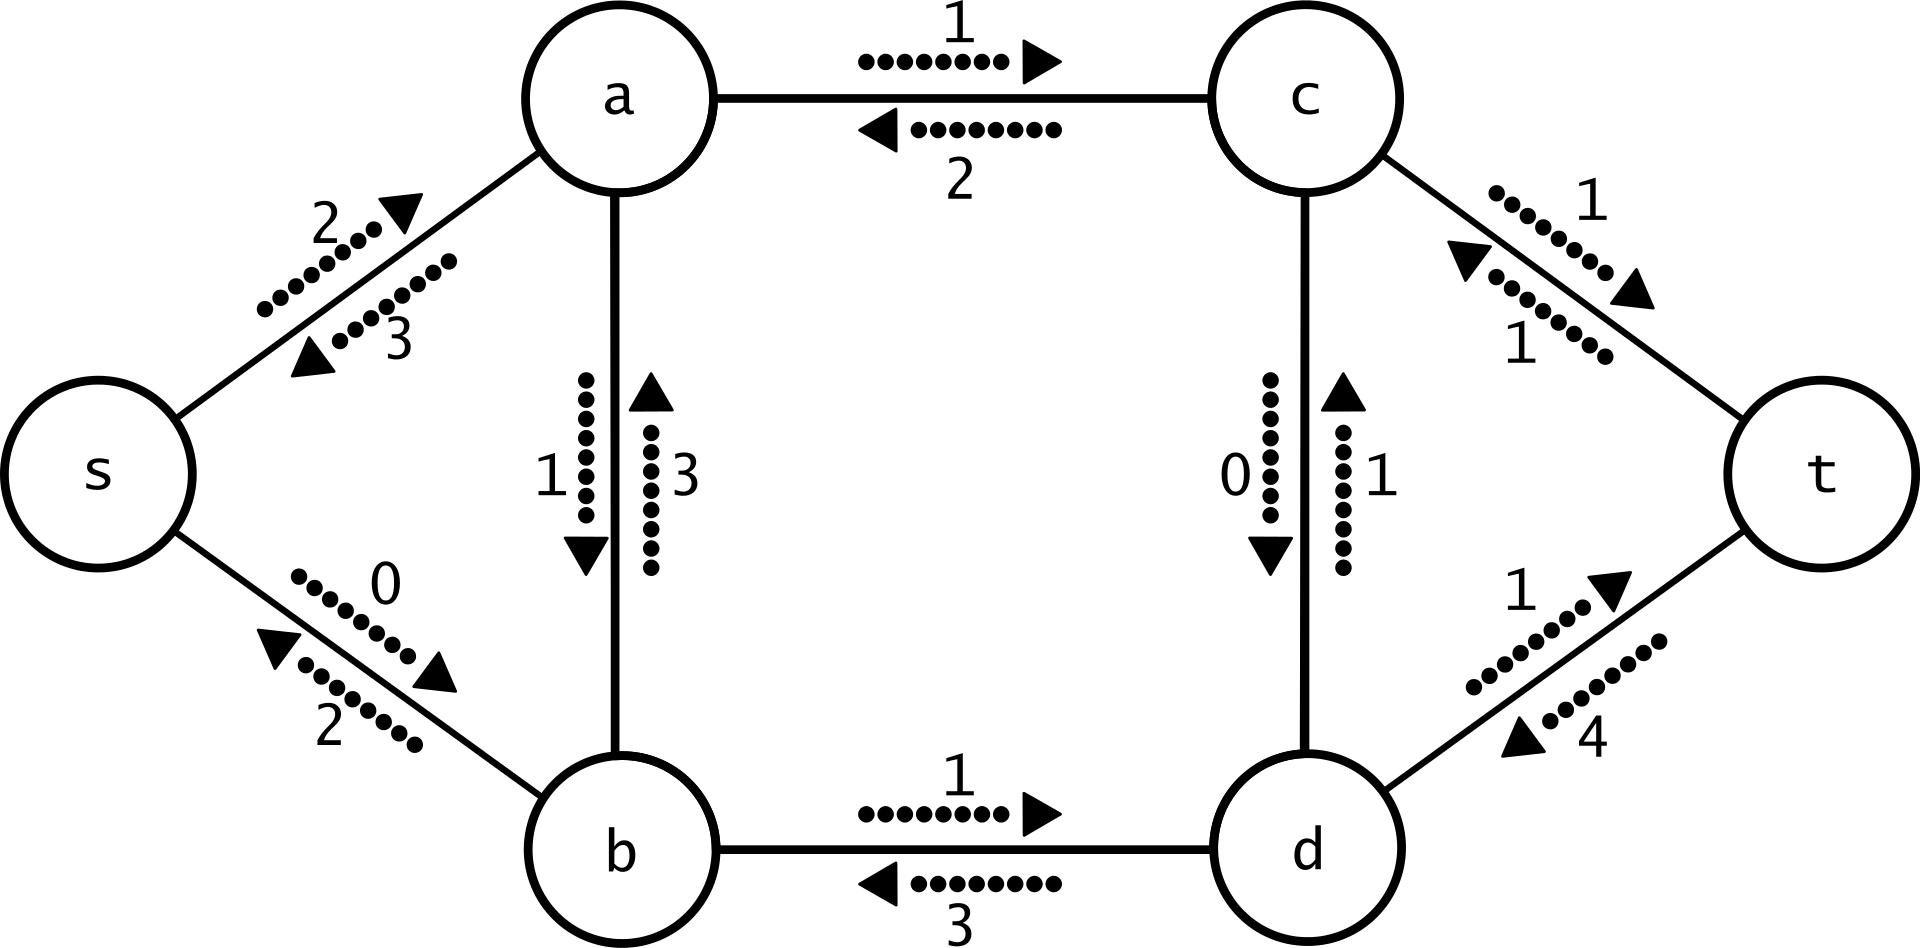
\includegraphics[scale=.06]{images/residual.png}
\end{center}

\subsubsection*{Max Flow Min Cut Theorem}
The size of the maximum flow in a network equals the capacity of the smallest (s,t)-cut, where and (s,t)-cut partitions the vertices into two disjoint groups L and R such that s (start) is in L and t (goal) is in R.

\subsubsection*{Bipartite Matching}
Explained by Example: list of boys, list of girls, if boy likes girl, a direct edge exists from boy to girl. Is there a perfect matching?
Create source node $s$ and sink node $t$, $s$ has outgoing edges to all the boys, and $t$ has incoming edges from all the girls. Give every edge a capacity of one (obviously). A flow exists if there is a flow into $t$ with size equal to number of couples. 

%%%%%%%%%%%%%%%%%%%%%%%%%

\section*{Computational Complexity}
We use Computational Complexity to determine classifications for our algorithms to know if they are feasible. 

\subsection*{Decision vs. Search Problems}
\textbf{Decision Problem: }Computational problem that answers ``Yes'' or ``No''. Our input can be any possible string (binary, ASCII), and it will answer either 0 or 1 depending upon weather the solution is correct or not. This type of problem determines our classes.\\
\textbf{Search Problem: }Computational problem tasked with not if a solution exists, but what one is. Decision problems can be derived from Search problems which are generally always more difficult. 

\subsection*{Classifications}
\begin{itemize}
\item \textbf{P}: The set of all search problems that are solvable in a reasonable amount of time (Polynomial time).
\item \textbf{NP (Nondeterministic Polynomial)}: The set of all search problems whose solution can be checked in Polynomial time (includes P) - there might exist search problems whose solutions can not be checked in Polynomial time. A solution may not necessary be found in a reasonable amount of time ($2^n$ and $n!$ algorithms can be in NP). Called NP because if you had the power to guess correct every time it would work in Polynomial time, making it non-deterministic. Should be called ``Guessing in P''.
\item \textbf{NP-Hard:} Any problem in NP can be reduced to this problem in Polynomial time, so it is at least as difficult or ``hard'' as any NP problem. The Halting Problem is NP hard and also impossible to solve in a finite amount of time, so this idea is not always practically useful for reductions. Most NP-Hard problem are NOT in NP, but those that are, are NP-Complete.
\item \textbf{NP-Complete: }Problem that is not only as hard as every problem in NP, but is also in NP. (NP-Hard and in NP). Any NP problem can be reduced to one of these in Polynomial time. It is often useful to prove the difficulty of problems. These are the hardest problems in NP and the reason why P = NP can revolutionize things. 
\end{itemize}
\begin{center}
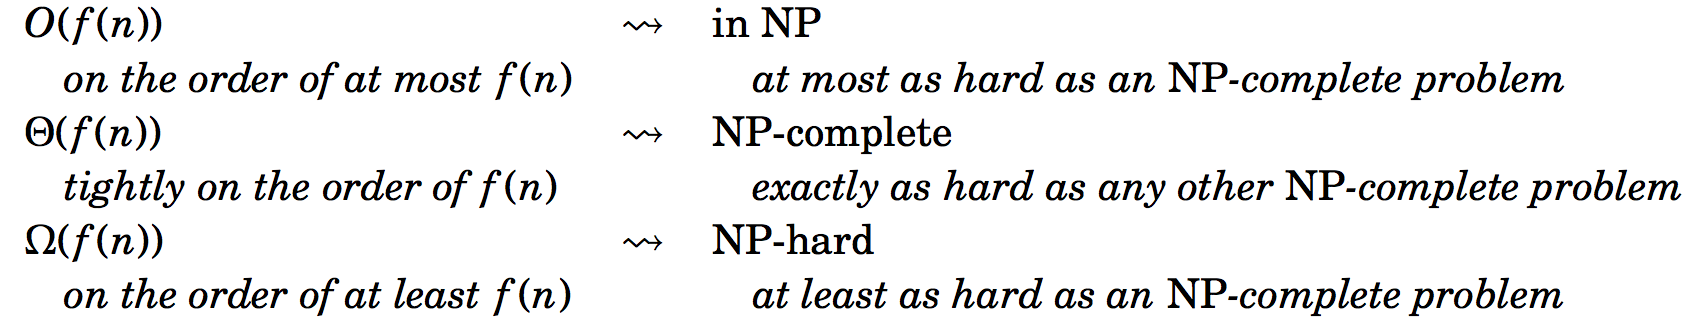
\includegraphics[scale=.25]{images/analogy.png}
\end{center}

\subsection*{Common NP-Complete Problems}
\begin{center}
\begin{tabular}{|c|c|}
    \hline
    Hard problems(NP-complete) & Easy problems (in P)\\
    \hline
    \hline
    3SAT & 2SAT, HORN SAT\\
    Traveling Salesman Problem & Minimum Spanning Tree\\
    Longest Path & Shortest Path\\
    3D Matching & Bipartite Matching\\
    Knapsack & Unary Knapsack\\
    Independent Set & Independent Set on trees\\
    Integer Linear Programming & Linear Programming\\
    Rudrata Path & Euler Path\\
    Balanced Cut & Minimum Cut\\
    \hline
\end{tabular}
\end{center}

\subsubsection*{Satisfiability (SAT)}
This is the prototypical NP-Complete problem that everything started from.
Say you have some Boolean expressions written using only AND, OR, NOT, variables, and parentheses (Example: $x_1 \land x_2 \lor x_3$). The SAT problem is given any one of these expressions, is there some assignment of TRUE and FALSE values to the variables that will make the entire expression TRUE? 
\subsubsection*{3SAT}
This is a stricter version of the SAT problem in which the statement is divided into clauses where each clause can have exactly 3 literals. (Example: $(x_1 \lor x_2 \lor x_3)\land(x_4 \lor x_5 \lor x_6)$). For these you want to find whether there exists values for $x_1 ... x_6$such that the boolean evaluates to TRUE.
\subsubsection*{CircuitSAT}
Given a circuit of logic gates with a single output and no loops find there a setting of the inputs that causes the circuit to output 1.
\subsubsection*{Integer Linear Programming} 
Solve a problem using linear objective function and linear inequalities, WHILE constraining the values of the variables to integers. 
\subsubsection*{Traveling Salesman Problem (TSP)}
Find the \textit{shortest path} in a graph that visits all the vertices exactly once before returning home. This comes from the idea of a traveling salesman wanting to efficiently visit all the cities to sell his wares. 
\subsubsection*{Rudrata/Hamiltonian Cycle}
Given a graph find if there a cycle that passes through each vertex exactly once, or report one doesn't exist. 
\subsubsection*{Rudrata/Hamiltonian Path}
Given a path starting at $s$ and ending at $t$ that goes through each vertex exactly once.
\subsubsection*{Independent Set}
Given a graph and a number $g$, the aim is to find $g$ vertices that are independent meaning that no two of which have share an edge. 
\subsubsection*{Graph 3-Coloring}
Given an undirected graph G = (V,E) find a valid 3-coloring C such that no two vertices sharing the same edge have the same color, or report that such an ordering doesn't exist. 


%%%%%%%%%%%%%%%%%%%%%%%%%

\section*{Reductions}
Reductions are an incredible useful tool for either turning a search problem we don't know how to solve into one we do, or proving that a search problem can not be solved or is hard to solve by reducing it to problem that is one of those two things.\\
- We know how to solve $B$ in a reasonable amount of time and we want to use this knowledge to solve $A$.\\
- We denote a reduction from $A$ to $B$ as $A \to B$. Difficultly flows in the direction of the arrow.\\
- If we can reduce our unknown problem $A$ into a known problem $B$ then $B$ must be as hard if not even harder to solve than $A$. A way to mathematically write this is $A \le_{p} B$. $A$ thereby provides a lower bound of hardness for $B$.\\ 
- Reduction can be composed as well: if you can reduce $A \to B$ and $B \to C$ then $A \to C$.\\
- Any search problem in NP can be reduced to an NP-Hard Problem in Polynomial Time but this is not always useful (like Halting Problem) \\
- Any search problem in NP can also be reduced to an NP-Complete Problem in Polynomial Time.\\
- Any problem that is NP-Complete is reducible to any other problem that is also NP-Complete which is very useful.
\subsubsection*{Reduction Tree}
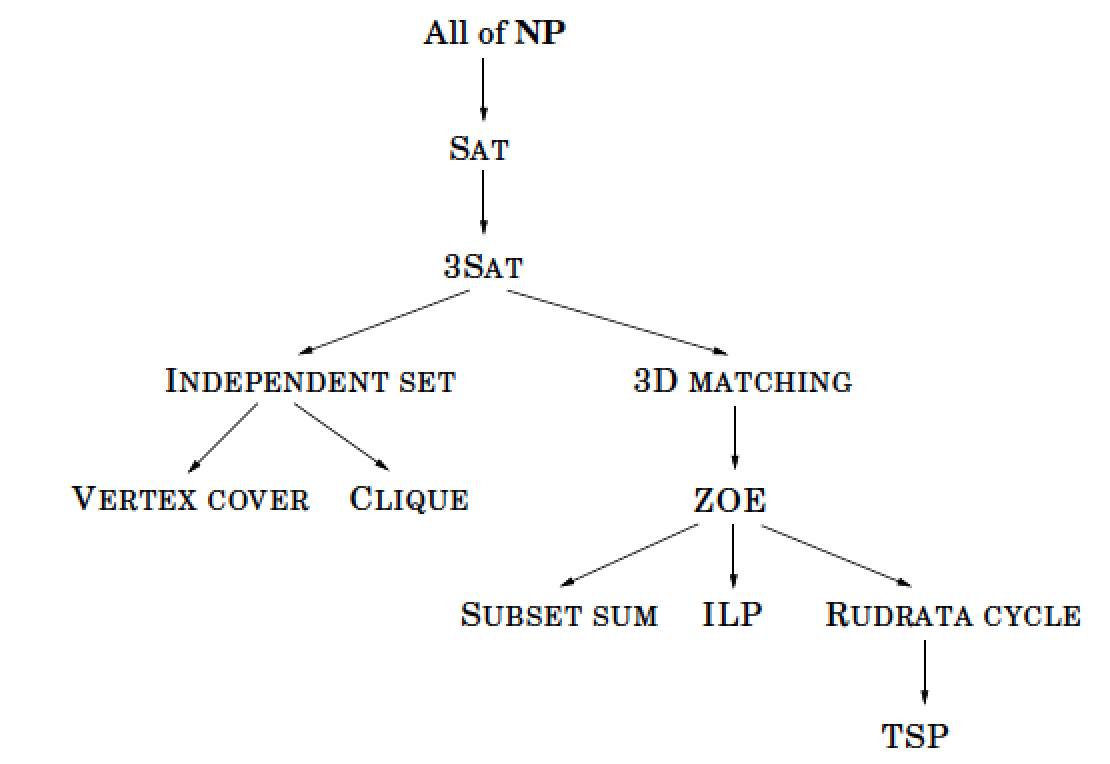
\includegraphics[scale=.4]{images/reductions.png}


%%%%%%%%%%%%%%%%%%%%%%%%%
\subsection*{Dealing with NP-Completeness}

\subsubsection*{Backtracking}
Backtracking is the idea of rejecting a portion of a solution that in some manner proves to be useless without fully processing it. Say if you find a violation of a certain criteria set in your algorithm, then you can stop, no longer process the children of that node and move up to another node to try its luck. It's not going to work anyways since it didn't work for the parent. \\
More abstractly, a backtracking algorithm requires a test that looks at a subproblem and quickly declares one of three outcomes:

\begin{itemize}
\item Failure: the subproblem has no solution. backtrack.
\item Success: a solution to the subproblem is found. 
\item Uncertainty: branch again and retry.
\end{itemize}

\begin{verbatim}
Start with some problem P0
Let S = {P_0}, the set of active subproblems 
Repeat while S is nonempty:
  choose a subproblem P ∈ S and remove it from S 
  expand it into smaller subproblems P_1, P_2, . . . , P_k 
  For each P_i:
    If test (P_i) succeeds: 
        halt and announce this solution
    If test (P_i) fails: 
        discard Pi Otherwise: add P_i to S
Announce that there is no solution
\end{verbatim}


\subsubsection*{Branch-and-bound}
Another technique in which you don't process off a whole portion of a tree because due to some formula you know it will not offer a more efficient solution. 
For example if you need to choose find a Hamiltonian path and you have thus far a path $A$ with weight 3 and another path $B$ with weight 7, given the information that the MST for the rest of the nodes for each path is of length 12, you can disregard the brute force calculation of the longer path, since it won't be better than what you already have.\\
Finding the lowerbound is the really tricky part. 
\begin{verbatim}
Start with some problem P0
Let S = {P0}, the set of active subproblems 
bestsofar = infinity 
Repeat while S is nonempty:
	choose a subproblem (partial solution) 
	P in S and remove it from S 
	expand it into smaller subproblems P_1, P_2, ..., P_k
	For each P_i:
		If P_i is a complete solution: update bestsofar
		else if lowerbound(Pi) < bestsofar: add Pi to S 
    return bestsofar
\end{verbatim}
%%%%%%%%%%%%%%%%%%%%%%%%%

\subsubsection*{Approximation Ratio}

Finding the OPT(I) is the challenging part, but it is always positive. 

For Minimization:
$\alpha_{A} = max (I)$ of $\frac{A(I)}{OPT(I)}$

For Maximization:
$\alpha_{A} = max (I)$ of $\frac{OPT(I)}{A(I)}$

Vertex Cover
Input: An undirected graph G = (V, E).
Output: A subset of the vertices S contained in V that touches every edge. Goal: Minimize |S|.

Special Case of Set Cover, works in $\O (log n)$


%%%%%%%%%%%%%%%%%%%%%%%%%

\section*{Machine Learning Algorithms}

Use big data set to train a classifier, which can then categorize new data.
Data partitions: take $80\%$ of data and use it as training, ie, feed into classifier both the data and expected result. use 20% for validation to get error rate and see how well you are performing.

Data is encoded as “features”, which is usually a vector of numbers, often normalized to floats between 0.0 and 1.0, These features are used to train the classifier.

\subsection*{K Nearest Neighbors}
We are working in a multidimensional space, with a dimension for each feature index. We then take all of our points and store them in some data structure that allows us to query for the nearest neighbors to an arbitrary point. The way the classification works is given a new point, we plot it, and get the K nearest neighbors to it. (Those neighbors are the test points we used to train the classifier.) Once we get those neighbors, we take a majority vote on their labels and figure out what this new unseen point actually is.\\

A small example: Imagine you are applying to a credit card. They ask for you age, income, and number of credit cards. From this, they create a 3 dimensional feature: {age, income, count}. The company takes your data and checks their classifier. The classifier plots your point and sees that you fall right in the middle of a cluster of people who always pay their bills on time. You are then judged as a good client.

This is our classify algorithm: \\
Runs in $\theta(nd)$
\begin{verbatim}
def Classify(x):
  set i* = 1
  for i - 2, 3,..., n:
    if ||x-x_i|| < ||x-x_i*||, set i* = i
  return y_i*
\end{verbatim}

Now to make this more accurate by using a voting system:\\

Given x, we compute the distance from x to each observation in the training set, and then keep the k
closest observations. Intuitively, the class of each of them gives a plausible suggestion for the class
of x. Therefore, we can treat each as a vote for the class of x. We take these k votes, find which
class received the most votes, and classify x with this class. In many applications, this improves
the accuracy of the nearest neighbor classifier by “smoothing” out the classifier’s predictions.\\

For boolean classification, it is often convenient to choose
k to be odd, to avoid ties.\\

Runs in $\theta(n(d + lg k))$ but for small values of k this is almost as fast as the classifier. 


%%%%%%%%%%%%%%%%%%%%%%%%%


%\rule{0.3\linewidth}{0.1pt}
\scriptsize

\end{multicols}
\end{document}
